\documentclass[../main.tex]{subfiles}
\begin{document}
\chapter{\textit{Risk \& security assessment} in infrastrutture cloud}
Lo sviluppo dei paradigmi distribuiti per la realizzazione di infrastrutture informatiche complesse, unito alla prassi del \textit{service-oriented computing}, ha portato con il passare del tempo allo sviluppo di una nuova filosofia: quella dell'\textit{as-a-service}\footnote{Fruizione di una risorsa come servizio}, che esprime tutta la sua essenza in un concetto del tutto innovativo: il \textit{cloud computing}.

Questo primo capitolo illustrerà il \textit{cloud computing} in relazione al contesto storico-evolutivo in cui si è sviluppato, soffermandosi sulle tecnologie di virtualizzazione dei sistemi e di contenimento delle applicazioni di cui si avvale.
Verranno discussi gli aspetti di sicurezza, evidenziando i punti di forza ed effettuando un'analisi dei rischi in relazione ai vari modelli di servizio e di \textit{deployment}.

\section{\textit{Outsourcing} dei servizi}
Al fine di contenere i costi di gestione e di manutenzione dell'apparato infrastrutturale, si è diffusa tra le aziende l'abitudine di esternalizzare i servizi presso fornitori di terze parti specializzati \cite{OutsourcingCloudDhardBalakrishnan}.
Per \textit{outsourcing} si intende \textit{l'atto di delegare o trasferire le decisioni di carattere informatico, i processi di business, le attività interne o i servizi a fornitori esterni, che si occuperanno di svilupparli, gestirli, amministrarli, in relazione al risultato e alle prestazioni accordate per mezzo di un contratto} \cite{OutsourcingCloudDhardBalakrishnan}.
All'inizio del fenomeno dell'\textit{outsourcing} ci si concentrava sulle problematiche relative alla fornitura interna od esterna dei servizi e su quali di questi dovessero essere forniti internamente o esternamente. Più tardi, nel 1989, una decisione strategica di Kodak portò a un approccio differente, indirizzando l'argomento verso un design verticalizzato \cite{OutsourcingCloud2}.

\section{Benefici e rischi dell'\textit{outsourcing}}
Lo scopo di un'azienda è innanzitutto quello di poter fornire servizi competitivi nel proprio ambito di competenza; spesso la  manutenzione dell'apparato informatico costituisce un costo aggiuntivo difficilmente tollerabile.
Non essendo tutte le aziende incentrate sullo sviluppo del software e sulla manutenzione degli apparati informatici, è impensabile che ognuna di esse possa disporre di un reparto informatico sufficientemente evoluto da poter garantire un'efficiente gestione dei servizi IT.
L'esternalizzazione permette a queste aziende di concentrarsi maggiormente sul proprio business, con garanzie di efficienza e produttività.
Per questo motivo i servizi di carattere generale che richiedono un impegno economico non trascurabile (es. gestione dei pagamenti, dei centralini telefonici, delle e-mail in uscita, hosting di siti e servizi web, storage) vengono generalmente demandati a terze parti \cite{OutsourcingCloud}.
Il proliferare di fornitori di servizi in outsourcing ha provocato una notevole concorrenza nel settore e l'abbassamento dei prezzi.
Dal \cite{OutsourcingCloud} possiamo inoltre ricavare le principali motivazioni (e i benefici) che spingono le organizzazioni ad esternalizzare i servizi:
\begin{enumerate}
\item \textit{Contenimento dei costi}
\item \textit{Velocità nel ciclo di sviluppo}
\item \textit{Garanzia di prestazioni e di qualità}
\item \textit{Servizio distribuito geograficamente}
\item \textit{Contratti di affitto strutturati e dimensionati}
\end{enumerate}
Occorre però anche individuare e valutare i possibili rischi dell'outsourcing: il problema principale è costituito dalla distinzione tra outsourcing parziale e outsourcing totale e dai guadagni che l'esternalizzazione dei propri servizi può effettivamente portare, in relazione anche al contesto nella quale viene effettuata.
Solo recentemente, infatti, si è sviluppata la consapevolezza che un contratto tra le parti di per sé non è in grado di coprire completamente la complessità del processo di outsourcing. Questo è particolarmente vero soprattutto nell'ottica in cui il bene da esternalizzare sia un servizio IT, concetto volatile per definizione, il quale richiede una certa flessibilità in funzione della sua elevata dinamicità \cite{OutsourcingCloud2}.


\section{Definizione di cloud computing}
Il cloud computing è la più recente tecnica di outsourcing, parziale o totale, delle procedure IT ed è caratterizzato dalla possibilità di usufruire di piattaforme e tecnologie mature e altamente scalabili.
Per questa ragione pone delle sfide importanti ai metodi tradizionali di outsourcing e ha un impatto notevole sulle trasformazioni che il concetto di "esternalizzazione del servizio" sta subendo \cite{OutsourcingCloud}.
Se da una parte, infatti, i clienti possono usufruire di servizi efficienti al massimo della flessibilità monetaria (modelli \textit{pay-per-use}), è altrettanto vero che la richiesta di innovazione è in crescita, a causa anche della necessità di soddisfare le specifiche esigenze di ogni consumatore \cite{OutsourcingCloud2}.

La definizione presa in considerazione in questo elaborato di tesi è quella fornita dal NIST\footnote{National Institute of Standards and Technology} nel documento NIST SP 800-145: The NIST Definition of Cloud Computing \cite{NISTCloud}.
Il termine \textit{cloud computing} indica un insieme di tecnologie informatiche che permettono l'accesso on-demand a un pool di risorse condivise (reti, server, storage, potenza computazionale, applicazioni, servizi) messe a disposizione su una rete eterogenea distribuita tramite tecniche di astrazione (es. APIs), virtualizzazione e contenimento, rilasciabili celermente con il minimo effort e la minima interazione da parte sia dell'utente, sia del fornitore di servizio. %ELIA il minimo effort da parte di chi? dell'utente? io scriverei il minimo impegno da parte dell'utente
%sia da parte dell'utente che da parte del provider di servizi, l'automazione è totale. Se digitalocean, per esempio, dovesse stare dietro a tutti i clienti, sarebbe una follia. Quindi minimo effort da parte di entrambi...
L'obiettivo principale del cloud computing è proprio quello di fornire le basi tecniche per soddisfare le esigenze di flessibilità e dinamicità del cliente.
Mentre in passato le risorse fisiche per effettuare outsourcing venivano mantenute sia dal cliente che dal provider, con l'avvento del cloud computing si stabilisce un paradigma basato sulla fornitura di servizi asset-free \cite{OutsourcingCloud2}.
Il NIST \cite{NISTCloud} descrive il cloud computing come un modello composto di cinque caratteristiche essenziali, tre modelli di servizio e quattro modelli di deployment.
\subsection{Caratteristiche essenziali del modello cloud}
Sono ivi descritte le caratteristiche essenziali del modello cloud:
\begin{itemize}
\item \textit{On-demand, self-service} Un cliente deve poter ottenere il servizio richiesto automaticamente, senza bisogno di alcuna interazione umana con il fornitore.
Questo obiettivo viene spesso raggiunto tramite l'esposizione di interfacce pubbliche, talvolta integrate con interfacce grafiche. Il consumatore del servizio può utilizzare queste interfacce per realizzare infrastrutture e/o topologie di rete, effettuare il deploy di macchine autonomamente e realizzare meccanismi di automazione per le proprie applicazioni, al fine di conferire maggiore dinamicità e capacità di autoscaling al software cloud.\\Per raggiungere questo obiettivo si implementano generalmente varie soluzioni di emulazione e/o virtualizzazione (ad es. software-defined network, virtualizzazione tramite hypervisor, paravirtualizzazione).
\item \textit{Accesso alle risorse tramite la rete e meccanismi standard} per favorire l'interazione con dispositivi thin-client o thick-client eterogenei, ad esempio smartphone, notebook, dispositivi embedded. Ogni risorsa è contrassegnata da un identificatore univoco all'interno del sistema, ottenuto tramite meccanismi di hashing. Ad ogni risorsa sono poi associate delle azioni, che variano a seconda della tipologia della risorsa stessa.
\`E il caso per esempio dell'object-storage, un meccanismo di memorizzazione di file che astrae il file system e, basandosi su database non relazionali o key-value storage, consente di implementare per esempio la multi-tenancy. %ELIA avoja a note a piè di pagina che dovresti mette qui! SDN, paravirtualizzazione, almeno...
\item \textit{Resource pooling} Le risorse del fornitore sono raggruppate per servire clienti multipli utilizzando un modello multi-tenant, assegnando e rimuovendo le risorse fisiche e virtuali in modo dinamico in base alla richiesta del consumatore.
Ciò deve garantire inoltre un senso di trasparenza rispetto a dove sono effettivamente localizzate le risorse.
I consumatori sono in grado di accedere solo alle loro risorse, con la convinzione di essere gli unici utilizzatori del servizio. 
\item \textit{Rapid elasticity} Le risorse devono poter essere ottenute e rilasciate in modo elastico (in alcuni casi anche automaticamente, per consentire ai processi di scalare orizzontalmente in modo automatico per soddisfare le richieste). Il cliente deve poter vedere risorse in quantità illimitata e approviggionabili in qualunque momento e in qualunque quantità.
Ciò favorisce, ad esempio, la scalabilità orizzontale. In qualunque momento colui che usufruisce del servizio può allocare le risorse necessarie a soddisfare le proprie esigenze, in funzione dell'aumento della complessità computazionale o del carico di rete.
\item \textit{Service metering} I sistemi cloud devono poter controllare e ottimizzare l'uso delle risorse facendo uso di capacità di misurazione, a un livello di astrazione appropriato a seconda del tipo di servizio (es. quantità di storage, potenza computazionale, banda, account utente attivi). L'uso delle risorse deve quindi poter essere monitorato, controllato, riportato, fornendo trasparenza sia per il provider che per il cliente.
Questa caratteristica è forse la più evidente in un servizio cloud, poiché grazie a ciò è possibile realizzare delle politiche economiche \textit{pay-as-you-go}.
Attraverso il metering non solo è possibile conoscere il carico a cui è sottoposta l'infrastruttura cloud, ma è anche possibile effettuare misurazioni sulle singole tenancy fatturando al consumatore soltanto ciò che ha effettivamente utilizzato.
Questo si traduce in maggiore convenienza economica, soprattutto in un'ottica di outsourcing.
\end{itemize}
\subsection{Modelli di servizio}
In figura \ref{fig:modelliservizio} sono mostrati i modelli di servizio per i servizi cloud, per come presentati in \cite{NISTCloud}.
\begin{figure}[H]
\centering
\makebox[\textwidth]{
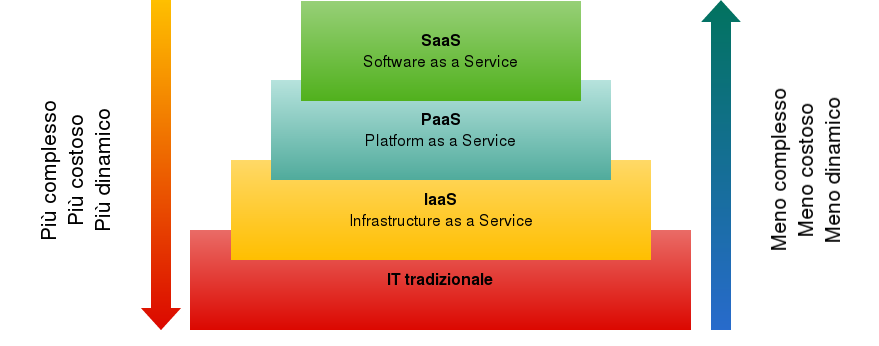
\includegraphics[width=\textwidth]{immagini/IAASPAASSAAS.png}
}
\caption{Modelli di servizio}\label{fig:modelliservizio}
\end{figure}

\begin{itemize}
\item \textit{\textbf{IaaS} - Infrastructure as a Service} Il paradigma IaaS fornisce le risorse fondamentali di calcolo (potenza computazionale, storage, reti, ecc.), permettendo al cliente di installare ed eseguire software arbitrario, che può includere sistemi operativi e applicazioni. Il cliente non gestisce né controlla l'infrastruttura cloud sottostante, ma ha il possesso dei sistemi operativi, della rete (con eventuali restrizioni), lo storage e le applicazioni deployate.
\`E il modello più versatile, ma anche il più costoso e difficile da amministrare.
L'infrastruttura cloud è formata da una o più macchine fisiche che forniscono le risorse hardware per costituire un livello di astrazione nel quale verrà effettuato il deploy di un pool di macchine virtualizzate.
L'orchestrazione dei processi di business all'interno di una IaaS è spesso demandata a un \textit{middleware} (es. Open Stack, Open Nebula, oVirt), che si occupa di gestire i servizi fondamentali per il sostentamento dell'infrastruttura (es. networking, storage, hypervisor).
\item \textit{\textbf{PaaS} - Platform as a Service} Il paradigma PaaS fornisce al cliente la possibilità di effettuare il deploy sul cloud di un'applicazione, proprietaria o acquisita, creata utilizzando linguaggi di programmazione, le librerie e i servizi supportati dal fornitore o che il fornitore mette spontaneamente a disposizione. Il cliente non ha né il controllo, né il possesso dell'infrastruttura cloud sottostante, ma può amministrare solamente le proprie applicazioni e personalizzare in modo limitato la configurazione dell'ambiente.
Esempi di PaaS sono Open Shift, Cloud Foundry, IBM Bluemix.
\item \textit{\textbf{SaaS} - Software as a Service} Il paradigma SaaS fornisce al cliente il mero utilizzo di un'applicazione in esecuzione su un'infrastruttura cloud. Le applicazioni sono accessibili tramite dispositivi client di vario tipo, interfacce thin-client come il browser web o l'interfaccia utente di un programma.
Il cliente non amministra né controlla l'infrastruttura cloud sottostante ma ha accesso solo a specifiche impostazioni dell'applicazione in uso \cite{NISTCloud}.
\`E il più alto livello di astrazione: le applicazioni sono fornite come servizio tramite il world-wide-web. 
Esempi di SaaS sono Microsoft Office 365, Google Docs, Share Latex, Odoo (OpenERP).
\end{itemize}
\subsection{Modelli di deployment}
\begin{itemize}
\item \textit{Private cloud}
Infrastruttura cloud fornita per l'utilizzo di un'unica organizzazione comprendente più utilizzatori. Può essere di proprietà, gestione e utilizzo dell'organizzazione stessa, di una terza parte o di entrambe \cite{NISTCloud}.
L'hardware può risiedere all'interno della struttura dell'organizzazione o all'esterno.
Un'applicazione possibile per una private cloud potrebbe essere quella del \textit{desktop as a service} in VDI\footnote{VDI - Virtual Desktop Infrastructure}: in un'ottica di allestimento di uffici, si possono virtualizzare gli endpoint in modo da sostituire i computer dei dipendenti di un'azienda con dispositivi thin-client a basso costo.
\item \textit{Community cloud}
Infrastruttura cloud fornita per uso esclusivo di una comunità di utenti appartenenti ad organizzazioni con gli stessi interessi e requisiti (es. obiettivi, esigenze funzionali, esigenze di sicurezza, politiche). Può essere di proprietà, gestione e utilizzo di una o più organizzazioni della community, una terza parte o entrambe le cose \cite{NISTCloud}.
\item \textit{Public cloud}
Infrastruttura cloud predisposta e ideata per l'uso pubblico. Può essere di proprietà e/o gestione di aziende, istituti accademici, organizzazioni governative o una combinazione di queste \cite{NISTCloud}.
\`E l'implementazione più comune: le risorse e i servizi vengono resi disponibili al pubblico su una rete (es. internet) e il provider ne predispone delle metriche per la fatturazione per l'uso.
\item \textit{Hybrid cloud}
Infrastruttura cloud formata da una composizione di due o più infrastrutture cloud (private, community o pubbliche). Le singole infrastrutture rimangono entità uniche e distinte, ma sono legate tra loro dall'utilizzo di una tecnologia standard o proprietaria che permette la portabilità delle applicazioni e dei dati \cite{NISTCloud}. Ciò contribuisce ad aumentare la flessibilità del cloud, utilizzando le peculiarità di ciascuna delle tipologie sopra descritte.
\end{itemize}
\begin{figure}[H]
\centering
\makebox[\textwidth]{
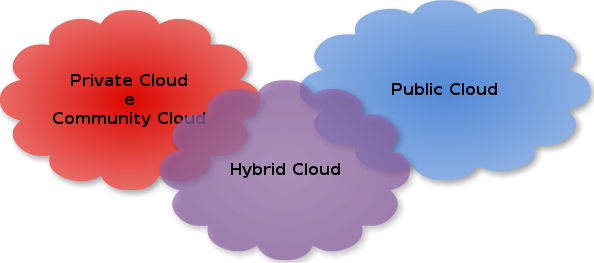
\includegraphics[width=\textwidth]{immagini/privatepublichybrid.png}
}
\caption{Modelli di deployment}\label{fig:modellideployment}
\end{figure}

\section{Valutazione della sicurezza e classificazione dei rischi in ambito cloud}
L'utilizzo di un'infrastruttura cloud come servizio pone problemi di sicurezza non indifferenti per le aziende, soprattutto per quanto riguarda l'utilizzo di applicativi business-critical sul cloud.
Al giorno d'oggi, garantire la sicurezza sul cloud è difficile, se non impossibile, perché ogni livello di servizio (IaaS, PaaS, SaaS) necessita di un proprio livello di sicurezza, che deve essere implementato in base alle esigenze del consumatore del servizio e alle caratteristiche dell'applicativo e del servizio in questione.
I servizi cloud hanno architetture differenti, basate sui servizi che devono fornire. I dati sono generalmente tenuti in datacenter centralizzati, che dispongono di un'ingente quantità di storage, ed elaborati in server distribuiti geograficamente. Per questo motivo, è importante per il cliente potersi fidare del proprio provider, sia per quanto riguarda la disponibilità dei dati, sia per la loro sicurezza.
L'unico punto di riferimento in questo senso è il contratto di SLA\footnote{Service Level Agreement, documento che definisce le relazioni tra fornitore e cliente}.
Esso deve essere formulato in modo adeguato, deve descrivere diversi livelli di sicurezza e la relativa complessità e consentire al cliente di comprendere le politiche di sicurezza implementate ai fini dell'erogazione del servizio \cite{CloudSecurityIssues}.




\subsection{Sicurezza a livello di infrastruttura}

Nella tabella \ref{tab:cloud_security_assessment_tab_infr} sono descritte le differenze tra gli \textit{asset} da proteggere in caso di infrastrutture cloud e in infrastrutture tradizionali.

\begin{table}[h]
\centering
\begin{tabular}{| m{2cm}| m{5.6cm} | m{5.6cm} | }
\hline
\textbf{Layer di protezione} & \textbf{Infrastrutture tradizionali} & \textbf{Infrastrutture Cloud} \\ \hline

Sicurezza fisica & Dispositivo, \textit{media}, ambiente & Dispositivo, \textit{media}, ambiente \\ \hline

Sicurezza di rete & Struttura di rete tradizionale, dispositivi di rete tradizionali, dispositivi di sicurezza tradizionali & struttura di rete virtualizzata, dispositivi di rete virtualizzati \\ \hline

Sicurezza dell'host & Sistema operativo, Database & Macchina virtuale \\ \hline

Sicurezza di risorse astratte & Nessuna & Host, Macchina virtuale, Monitor delle macchine virtuali, Software di gestione delle macchine virtuali, Cluster di macchine virtuali \\  \hline

\end{tabular}
\caption{Paragone degli oggetti da proteggere a livello infrastruttura in sistemi tradizionali e sistemi informativi sul cloud \cite{CSAssessmentSystemCG}}
\label{tab:cloud_security_assessment_tab_infr}
\end{table}

Andiamo ora a descrivere più dettagliatamente gli \textit{asset} specifici per le infrastrutture cloud.

\subsubsection{Network security}
Trattando la parte di sicurezza nelle reti, occorre considerare le notevoli differenze tra i modelli di deployment pubblico e privato.  
Infatti, trattando la casistica del cloud privato, non vi sono grandi considerazioni da fare per quanto riguarda attacchi, vulnerabilità o cambiamenti dipendenti dal fatto che ci si trovi in un'architettura cloud, piuttosto che in un'architettura classica \cite{CloudSecurityBook}.
Prendendo in considerazione il cloud pubblico, invece, i requisiti di sicurezza hanno un risvolto importante anche sulla struttura della topologia di rete. In particolare, bisogna considerare le modalità di interazione tra la propria topologia di rete e quella del cloud provider \cite{CloudSecurityBook}. Ci sono in particolare quattro rischi significativi relativi a:
\begin{itemize}
\item \textit{Confidenzialità e integrità dei dati relativi all'organizzazione, quando in transito}.
Il rischio di violazione della confidenzialità può essere sempre mitigato con la cifratura e la firma digitale, rendendo difficoltoso il tampering delle informazioni. Una delle tecniche più banali è l'utilizzo di HTTPS al posto di HTTP.
%ELIA il tampering? explain pls
\item \textit{Controllo degli accessi (autenticazione, autorizzazione, auditing) sulle risorse}. Il fatto che i dati siano esposti su Internet, apre un grande rischio sulla possibilità che essi possano essere oggetto di attacco ed essere consultati da persone non autorizzate. Da questo punto di vista ci sono ben poche difese: non è di fatto possibile effettuare attività di auditing sulle operazioni che il cloud provider compie. Non c'è inoltre controllo sulle capabilities di rete e sui router interposti tra gli endpoint di una comunicazione.
Questo provoca una forte limitazione nelle indagini forensi: la maggior parte delle volte il Service Level Agreement impedisce ai fornitori del servizio di divulgare informazioni riguardanti il traffico di rete, in quanto potrebbe contenere dati relativi ad altri clienti. Lo stesso vale per i log, il cui accesso è consentito in modo limitato.
\item \textit{Disponibilità delle risorse esposte su internet}. Ciò potrebbe corrispondere a varie casistiche, ad es. hijacking dei prefissi BGP\footnote{\textbf{Border Gateway Protocol}: è un protocollo di routing usato per interconnettere i router di confine di \textit{autonomous system} diversi}, configurazioni errate sul livello di rete, attacchi ai DNS\footnote{\textbf{Domain Name System}: è un sistema distribuito utilizzato per la risoluzione di nomi dei nodi della rete in indirizzi IP e viceversa} Molte di queste capabilities non sono a disposizione del cliente.
\item \textit{Sostituzione delle zone di rete con i domini}
Il modello di separazione delle zone di rete nel cloud è stato sostituito da una separazione in domini logici ("security groups", "security domains"). Non esiste più il concetto di separazione fisica; lo stack di rete è simulato in software (SDN, Software-defined Network) e si appoggia sullo stesso server fisico. La separazione logica è quindi a livello di host, ed è gestita dagli hypervisors di virtualizzazione.
Sebbene molti provider forniscano la possibilità di dividere la rete in zone, non è detto che a ciò non corrispondano misure di sicurezza adeguate \cite{CloudSecurityBook}.
\end{itemize}
\subsubsection{Host-security}
Anche in questo caso, le problematiche riguardano soprattutto la casistica del cloud pubblico.
Il cloud computing deve tutta la sua forza al concetto di elasticità, tuttavia questo porta a nuove sfide dal punto di vista della sicurezza; la gestione delle vulnerabilità e delle patch è molto più difficile rispetto ad un ambiente tradizionale. Il cloud è basato su numerosi nodi di \textit{compute} ugualmente strutturati che, combinati anche all'omogeneità dei sistemi operativi impiegati dai sistemi operativi guest, causano un'amplificazione notevole del propagarsi dell'effetto di una vulnerabilità.
%ELIA pure questa è arzigogolata forte, c'ho messo due minuti a cercare di capirla :)
Prima di fare considerazioni sull'offerta di sicurezza del provider, bisogna perciò capire come esso stia implementando il \textit{layer} di sicurezza anche in relazione alle tecnologie di virtualizzazione utilizzate \cite{CloudSecurityBook}.
A livello \textit{IaaS} possiamo trattare la sicurezza degli host categorizzandola in:
\begin{itemize}
\item \textit{Sicurezza del software di virtualizzazione}, ovvero il layer che si trova appena sopra il bare-metal e che fornisce ai consumatori del servizio la possibilità di creare e distruggere macchine virtuali. La virtualizzazione può essere raggiunta a livello di sistema operativo con isolamento a livello kernel (ad es. i container di Solaris, le jail di BSD, container LXC), con paravirtualizzazione (ad es. Xen), con hypervisor di virtualizzazione (ad es. Xen, vMware, Linux KVM, Microsoft Hyper-V). Il layer di virtualizzazione deve essere messo in sicurezza e non può essere gestito dal cliente \cite{CloudSecurityBook}.
Un hypervisor vulnerabile, per esempio, potrebbe esporre i domini interni ad utenti malevoli. 
\item \textit{Sicurezza del sistema operativo guest}, rappresenta la singola istanza, fornita sopra al layer di virtualizzazione, è totalmente gestita dal cliente.
Bisogna però considerare che, generalmente, le immagini utilizzate per la creazione delle istanze sono fornite direttamente dal provider. Per questo motivo esse contengono gli applicativi software installati dallo stesso (che potrebbero potenzialmente contenere trojan-horse o altri tipi di malware) e spesso sono equipaggiate con vari script e metodi di automazione \cite{CloudSecurityBook}.
La protezione del sistema operativo guest, inoltre, comprende una serie di raccomandazioni:
\begin{itemize}
\item Protezione delle chiavi utilizzate per gestire la macchina (es. chiavi SSH)
\item Protezione e patching dei servizi vulnerabili sulle porte standard
\item Protezione dagli hijack sugli utenti creati di default, in modo particolare in presenza degli script di automazione di cui sopra
\item Protezione delle macchine guest con soluzioni di host-firewalling, in aggiunta alle normali precauzioni prese dal provider di infrastruttura
\item Protezione delle macchine guest con soluzioni di host-IDS\footnote{Host Intrusionn Detection System}
\item Auditing e logging delle attività sul sistema
\item Messa in sicurezza e isolamento delle eventuali chiavi di cifratura
\end{itemize}
\end{itemize}
\subsection{Sicurezza a livello di piattaforma}
Le organizzazioni potrebbero utilizzare fornitori di servizi PaaS per ospitare applicativi utilizzati internamente.
La raccomandazione è sempre quella di effettuare una valutazione dei rischi applicando gli standard di sicurezza in modo simile a quando si acquista un nuovo software fondamentale per fini aziendali.
La sicurezza nei servizi PaaS può essere inclusa in due livelli:
\begin{itemize}
\item Sicurezza della piattaforma PaaS
\item Sicurezza dell'applicativo del cliente
\end{itemize}
Generalmente il fornitore del servizio è responsabile esclusivamente per il primo layer, in quanto l'applicativo deployato dal cliente potrebbe far riferimento anche a servizi di terze parti.
Inoltre il provider è responsabile del monitoraggio di bug e vulnerabilità che potrebbero essere usate per attaccare la piattaforma e romperne il sandboxing, così come dell'auditing a livello di rete.
In un modello di fornitura multi-tenant, gli elementi più influenti dal punto di vista della sicurezza sono il contenimento e l'isolamento delle applicazioni \cite{CloudSecurityBook}.
L'accesso ai dati, infatti, deve essere ristretto solo a determinati utenti (gli aventi diritto di accesso agli stessi) e alle applicazioni da loro amministrati. Il modello di sicurezza è spesso proprietà intellettuale del provider, ed è essenziale per fornire una soluzione di sandboxing efficiente.

\subsection{Gestione dei dati e dello storage}

Il primo rischio nella gestione dei dati durante la loro trasmissione è l'inutilizzo - o l'utilizzo non idoneo - di un algoritmo di encryption robusto. Anche se ciò può sembrare ovvio, in realtà la crittografia del dato non è così semplice da ottenere.
Solitamente i provider cloud pubblici o privati suggeriscono di effettuare l'encryption dei dati memorizzati in modo permanente, tuttavia ciò causa notevoli problematiche nell'indicizzazione e nel reperimento dei dati, nonché nella loro elaborazione da parte di applicazioni cloud \cite{CloudSecurityBook}.
Una possibile soluzione potrebbe essere l'utilizzo di un algoritmo di cifratura omomorfico come quello proposto da Craig Gentry nel 2009 \cite{Gentry}, nella sua tesi di laurea all'Università di Stanford.
Inoltre bisogna considerare che i dati destinati ad essere utilizzati da un'applicazione cloud-based su servizi PaaS e SaaS pubblici sono mescolati con altri dati in un grande servizio di storage.
Sebbene i modelli multi-tenant siano strutturati per prevenire l'accesso non autorizzato a questi dati, ciò rappresenta comunque una minaccia da tenere in considerazione soprattutto in caso di attacco mirato alla piattaforma host \cite{CloudSecurityBook}.
Oltretutto, sia che i dati sul cloud siano memorizzati in modo cifrato o no, potrebbe essere necessario conoscere la loro localizzazione e il momento di creazione. Affinché ciò avvenga, non ci si può affidare ai tradizionali metodi di memorizzazione dei metadati: i dati possono essere spostati da un bucket di un provider e salvati in un altro bucket dello stesso provider, posto su un altro server, per esigenze di elasticità.
Affinché sia possibile effettuare l'attività di auditing, occorre perciò individuare un modo per effettuare la \textit{data-lineage}, ovvero il tracciamento del percorso di un determinato dato.
A ciò va anche associato il mantenimento dell'integrità del dato (il dato non deve essere stato modificato) e della sua provenienza (deve essere ancora computazionalmente accurato)\footnote{Ad esempio, se un'equazione finanziaria utilizza il dollaro come valuta, bisogna assicurarsi che il suo risultato non cambi in funzione della località geografica e del contesto in cui è posta la macchina di destinazione del dato generato da quell'equazione, la quale potrebbe considerare un cambio di valuta diverso da quello originale} \cite{CloudSecurityBook}.
Un rischio è quello della \textit{rimanenza del dato}, ovvero la parte residua di un dato nominalmente cancellato o rimosso causata da un dato lasciato intatto da un'operazione di eliminazione o dalle proprietà fisiche del dispositivo di memorizzazione.
Essa potrebbe causare la rivelazione di informazioni sensibili, ed essere esposta all'uso di una parte non autorizzata.
Delle azioni di mitigazione in caso di situazioni di questo tipo potrebbero essere:
\begin{itemize}
\item Cancellazione totale ed eradicazione del dato dal dispositivo di memorizzazione prima del suo riutilizzo, quando l'ambiente fornisce un livello di protezione accettabile dei dati rimossi (tutte le memorie interne, i buffer e la memoria riutilizzabile devono essere cancellate definitivamente per la preservazione delle informazioni memorizzate precedentemente)
\item Sanitizzazione del dato, nel caso in cui l'ambiente non fornisca un livello accettabile di protezione per i dati cancellati.
\end{itemize}
\subsubsection{Dati del provider e relativa sicurezza}
Oltre ai dati dei clienti, un provider deve proteggere anche i metadati ad essi relativi. \`E importante considerare come questi metadati vengono conservati ed eventualmente protetti: essi descrivono in modo completo il processo di fruizione del servizio, aumentano all'aumentare dei dati e possono contenere informazioni sensibili.
Alcuni di questi metadati, inoltre, sono rilevanti anche dal punto di vista della sicurezza. A livello di rete, per esempio, potrebbero contenere le definizioni di firewall, IDS\footnote{Intrusion Detection System}, dati relativi ai flussi di routing, dati relativi agli incidenti informatici e ai relativi sistemi di gestione degli eventi (SIEM), soprattutto nel caso in cui questi componenti vengano forniti \textit{as-a-service} \cite{CloudSecurityBook}.
\paragraph{Storage-\textit{as-a-Service}}
Andiamo ora ad analizzare l'applicazione del paradigma CIA, che deve essere definito a livello di Service Level Agreement, per quanto concerne i servizi di Storage as a Service.
\subparagraph{Confidenzialità}
La confidenzialità dei dati in un cloud pubblico va analizzata secondo due aspetti principali: il controllo degli accessi e come i dati vengono effettivamente protetti sul server del fornitore di servizi.
Per quanto riguarda il primo aspetto, si deve tenere sempre presente che il provider utilizza generalmente meccanismi di autenticazioni deboli (nome utente e password) e il processo di controllo dell'accesso non avviene con la dovuta granularità (non sono quasi mai definiti più livelli di autorizzazione per l'accesso a una risorsa).
Il secondo aspetto, invece, riguarda più le modalità di conservazione del dato una volta caricato. La protezione del dato avviene tramite meccanismi di cifratura, che non sempre però sono implementati.
Il consumatore del servizio può in ogni caso costruire il suo meccanismo crittografico, da applicare prima del caricamento dei dati. Questo comporta però problematiche per altre funzionalità che il fornitore solitamente mette a disposizione (ad es. versionamento del file) \cite{CloudSecurityBook}.
Se la cifratura viene applicata, è utile conoscere anche il meccanismo con cui essa viene effettuata: non tutti gli algoritmi di cifratura lavorano allo stesso modo e in generale è sempre meglio evitare algoritmi proprietari \cite{CloudSecurityBook}.
\`E utile però far riferimento agli standard crittografici validati dalla comunità e agli algoritmi noti.
\`E sempre meglio appoggiarsi ad algoritmi di cifratura simmetrica\footnote{Tecnica crittografica che utilizza la stessa chiave per effettuare encryption e decryption del dato}, che è l'unica a poter garantire prestazioni efficienti anche in caso di file molto grandi.
\begin{figure}[H]
\centering
\makebox[\textwidth]{

\includegraphics[width=\textwidth]{immagini/CifraturaSimm.png}
}
\caption[Cifratura Simmetrica]{Cifratura Simmetrica: Alice e Bob scambiano un messaggio crittografato, ed effettuano le operazioni di cifratura e decifratura con la stessa chiave \textit{k}}\label{fig:cifraturasimmetrica}
\end{figure}

Al contrario, la cifratura a chiave pubblica\footnote{Tecnica crittografica che utilizza due chiavi diverse (pubblica e privata) legate da una relazione matematica per effettuare le operazioni di cifratura e decifratura} non è in grado di garantire la stessa efficienza per questo caso d'uso \cite{CloudSecurityBook} (mentre ad esempio si rivelano efficaci per il controllo degli accessi).

\begin{figure}[H]
\centering
\makebox[\textwidth]{

\includegraphics[width=\textwidth]{immagini/CifraturaAsimm.png}
}
\caption[Cifratura asimmetrica o a chiave pubblica]{Cifratura asimmetrica o a chiave pubblica: Alice e Bob scambiano un messaggio crittografato. Alice cifra con la chiave pubblica di Bob \textit{k'} e Bob decifra con la sua chiave privata \textit{k''}}\label{fig:cifraturaasimmetrica}
\end{figure}

Un'altra importante considerazione riguardo la cifratura dei dati è relativa all'attore che effettivamente detiene le chiavi e il modo in cui le gestisce. In molte implementazioni le chiavi sono detenute dal fornitore del servizio, specialmente nel caso in cui la crittografia del dato è offerta come funzionalità integrata.
La gestione delle chiavi è inoltre un'attività molto complessa
\`E consigliato che il cliente abbia consapevolezza del contenuto del documento NIST 800-57 "Recommendation for Key Management" \cite{NISTKeys}, organizzato in tre parti: \cite{CloudSecurityBook}
\begin{itemize}
\item Parte generale
\item Raccomandazioni per l'organizzazione della gestione delle chiavi
\item Guida alla gestione delle chiavi nelle applicazioni
\end{itemize}
Inoltre, poiché la difficoltà di gestione delle chiavi è notevole, bisogna sempre tenere a mente che il cloud provider spesso non la effettua in modo opportuno: ad esempio è abitudine comune quella di cifrare i dati di tutti i clienti con un'unica chiave simmetrica.

\subparagraph{Integrità}
La confidenzialità dei dati non implica la loro integrità. La crittografia del dato, di per sé, non basta a verificare che il dato non sia stato manomesso.
Per questo fine si utilizzano i MAC\footnote{Message Authentication Code}. Il modo più semplice per usare i MAC è tramite cifratura simmetrica in modalità CBC\footnote{Cipher Block Chaining} per poi passare il dato crittografato a una funzione hash one-way. 
Il problema fondamentale del mantenimento dell'integrità dei dati sul cloud, è quello della verifica \cite{CloudSecurityBook}.
Per effettuare un controllo di integrità il cliente dovrebbe scaricare i dati in locale, verificarne l'integrità e ricaricare i dati sul cloud provider. Ciò, specialmente in caso di grandi moli di dati, può tradursi in un aumento spropositato dei costi, soprattutto in termini di banda e di utilizzo della rete.
Oltretutto spesso questi dati sono utilizzati dalle applicazioni cloud e quindi cambiano frequentemente e velocemente \cite{CloudSecurityBook}.

\subparagraph{Disponibilità}
Oltre a preservare confidenzialità e integrità, bisogna anche occuparsi della disponibilità dei dati \cite{CloudSecurityBook}.
Riguardo a ciò ci sono tre minacce principali:
\begin{itemize}
\item Attacchi basati sulla rete
\item Disponibilità e \textit{uptime} del provider
\item Non sempre viene fatto il backup dei dati
\end{itemize}
La disponibilità del dato viene garantita tramite la diffusione dello stesso su più località geografiche. Non sempre il fornitore del servizio garantisce questa funzionalità, ma qualora fosse stabilita a livello di \textit{Service Level Agreement} l'utente finale potrebbe contattare direttamente il server a lui geograficamente più vicino, con gli evidenti benefici sui tempi di latenza.

\subsection {La sicurezza nel \textit{Service Level Agreement}}
Grazie al documento \cite{CloudSecurityIssues} possiamo inoltre identificare i punti che un contratto di SLA deve sempre specificare:
\begin{itemize}
\item \textbf{Gestione delle performance}, ciò si traduce in attività di misurazione e monitoraggio, secondo delle metriche stabilite, affinché sia possibile garantire la disponibilità del dato.
\item \textbf{Politica di gestione degli incidenti}, il cui scopo è quello di minimizzare l'impatto di eventuali incidenti informatici o problematiche del servizio.
\item \textbf{Doveri e responsabilità del cliente}
\item \textbf{Garanzie e rimedi}
\item \textbf{Politiche di \textit{disaster-recovery} e continuità di business}
\item \textbf{Politiche e meccanismi di sicurezza}, in particolar modo:
\begin{itemize}
\item \textit{Accesso privilegiato alle risorse}: l'attività di elaborazione dei dati parzialmente incontrollata rispetto all'impresa che usufruisce dei dati, porta con se un elevato livello di rischio, poiché i servizi in \textit{outsourcing} spesso evitano i tradizionali controlli che i processi di business impongono.
\item \textit{Locazione dei dati}: Utilizzando il \textit{cloud}, probabilmente non sappiamo il luogo preciso in cui vengono conservati i dati. Ciò potrebbe essere causa di problemi dal punto di vista legale e in un'ottica operativa in ambito di informatica forense.
\item \textit{Segregazione dei dati}: i dati sul \textit{cloud} sono ospitati tipicamente in un ambiente condiviso, insieme ai dati di altri utenti. Le tecniche crittografiche possono essere efficienti, ma non sono sempre efficaci. Il \textit{cloud provider} dovrebbe fornire delle spiegazioni, su come sono stati progettati gli schemi di cifratura e i risultati di eventuali test effettuati da specialisti accreditati.
\item \textit{Recupero}: anche se non sappiamo dove si trovano i dati, il \textit{cloud provider} è tenuto ad informare le eventuali conseguenze sulla loro integrità e disponibilità in caso di disastro o incidente informatico. Occorre strutturare l'offerta in modo che sia presente un meccanismo di ridondanza e di \textit{disaster-recovery}.
\item \textit{Supporto investigativo}: l'attività di investigazione e di \textit{computer-forensics} potrebbe incontrare notevoli impedimenti in un'ottica di \textit{cloud computing}, a causa di come i dati vengono memorizzati. Gli stessi \textit{log} potrebbero essere sparsi su più \textit{host} e potrebbero non costituire un supporto totalmente affidabile per le attività investigative. La dinamicità e l'elasticità, per come descritte precedentemente, potrebbero costituire un ulteriore problema. 
\end{itemize}
\item \textbf{Terminazione del contratto}
\end{itemize}
\end{document}